\chapter{Projective Geometry}
\label{chap:projgeo}

\section{The Projective Space}

\subsection{Constructing the Projective Plane}

\subsection{Projective Spaces}

\begin{definition}
  Let $E$ be a finite dimwnsional vector space. The \textit{projective space} $P(E)$ deduced
  from $E$ is the set of all $1$ dimensional linear subspaces of $E$. \cite{audin}
\end{definition}

\begin{remark}
  The dimension of $P(E)$ is $dim$ $E-1$. If $E$ consists only of the point $0$, it does not
  contain any lines, and $P(E)$ is empty. Thus it shall be implicitly assumed that dim $E\ge1$.
  If dim $E=1$, $E$ itself is a line, and thus the set of linea comtains a unique element,
  $P(E)$ is a point.
\end{remark}

\subsection{Projective Subspaces}
A subset $V$ of $P(E)$ is a projective subspace if it is an image of a nonzero vector subspace
$F$ of $E$.

\begin{prop}
  Let $V$ and $W$ be two projective subspaces of $P(E)$.
  
  \begin{itemize}
    \item If dim $V$ + dim $W$ $\ge$ dim $P(E)$, then $V\cap U$ is not empty.
    \item Let $H$ be a hyperplane of $P(E)$, and let $m$ be a point not in $H$. Every
      line through $m$ intersects $H$ at a unique point.
  \end{itemize}

\end{prop}

\begin{proof}
  Let $F$ and $G$ be the vector subspaces of $E$ from which $V$ and $W$ were deduced, i.e.
  $V=P(F)$, and $W=P(G)$. The statement can be translated into vector subspaces as

  \begin{eqnarray*}
    & (\text{dim }F-1)+(\text{dim }G-1)\ge(\text{dim }E-1)\\
    \Longrightarrow& \text{dim }F+\text{dim }G\ge\text{dim }E+1
  \end{eqnarray*}

  We can use the linear algebraic properties to further deduce that:
  \[
    \text{dim }F+\text{dim }G=\text{dim }(F+G)+\text{dim }(F\cap G)
    \le\text{dim }E+\text{dim }(F\cap G)
  \]
  Therefore,
  \[
    \text{dim }(F\cap G)\ge1
  \]
  This can be translated back into projective geometry to conclude that $V\cap W$ is not empty.

  Now, to prove the second property, let $J$ be the vector hyperplane of which $H$ is image of.
  The point $m$ is the image of a line $l$ in $E$, not contained in the hyperplane $J$.
  The assertion, translated in terms of linear algebra, is that any plane $P$ containing $l$
  meets $J$ along a unique line. Since $l$ is not in $J$, we have $P+J=E$. Hence,

  \begin{eqnarray*}
    \text{dim }(P\cap J) &=& \text{dim }P+\text{dim }J-\text{dim }(P+J)\\
    &=& 2+\text{dim }E-1-\text{dim }E=1
  \end{eqnarray*}
\end{proof}

\subsection{Projective Transformations}

\begin{definition}
  Let $E$ and $E'$ be two vector subspaces, and $p:E-\{0\}\rightarrow P(E)$ and
  $p':E'-\{0\}\rightarrow P(E')$ be the two projections. A \textit{projective transformation}
  $g:P(E)\rightarrow P(E')$ is a mapping such that there exists a linear isomorphism
  $f:E\rightarrow E'$ with $p'\circ f=g\circ p$.
\end{definition}

\subsection{Homogeneous Coordinates and Projective Frames}

Given a basis of vector space $E$, the vectors in $E$ can be descirbed by their coordinates with
respect to the basis. 

\begin{definition}
  A point $m$ in $P(E)$ can be described by the nonzero vector that generates the line $m$. In a
  n-dimensional projective space $P(E)$, the $(n+1)$ tuples $[x_1,\ldots,x_{n+1}]$ and
  $[x'_1,\ldots,x'_{n+1}]$ represent the same point iff there exists a nonzero scalar $\lambda$
  such that $x_i=\lambda x'_i$ for all $i$.
\end{definition}

In a projective space $P(E)$ with dimension $n$, we actually need $n+2$ points to uniquely determine
the basis of the underlying space $E$, which will be proved in the next lemma. It will also
justify the next definition.

\begin{definition}
  If $E$ is a vector space of dimension $n+1$, a \textit{projective frame} of $P(E)$ is a set of
  $n+2$ points  $(m_0,\ldots,m_{n+1})$ such that $m_1,\ldots,m_{n+1}$ are the images of the
  vectors $e_1,\ldots,e_{n+1}$ in a basis of $E$, and $m_0$ is the image of
  $e_1+\cdots+e_{n+1}$.
\end{definition}

\begin{lemma}
  Let $(m_0,\ldots,m_{n+1})$ be a projective frame of $P(E)$. If the two bases of $E$
  $(e_1,\ldots,e_{n+1})$ and $(e'_1,\ldots,e'_{n+1})$ are such that $p(e_i)=p(e'_i)=m_i$ and
  $p(e_1+\cdots+e_{n+1})=p(e'_1+\cdots+e'_{n+1})=m_0$, then they are proportional.
\end{lemma}

\begin{proof}
  Consider the points $m_i$ of $P(E)$. Since the vectors $e_i$ and $e'_i$ both generate the line
  $m_i$, $e_i=\lambda_i e'_i$ for some nonzero $\lambda_i$. Using the $(n+2)-th$ point, we can
  conclude that 
  \[
    (e_1+\cdots+e_{n+1})=\lambda(e'_1+\cdots+e'_{n+1})
  \]
  Thus,
  \[
    \lambda_1e_1+\cdots+\lambda_{n+1}e_{n+1}=\lambda(e_1+\cdots+e_{n+1})
  \]
  As we are dealing with a basis, $\lambda_i=\lambda$. Thus two bases are proportional.
\end{proof}

\begin{prop}
  Let $P(E)$ and $P(E')$ be two projective spaces of dimension $n$. Any projectivve mapping from
  $P(E)$ to $P(E')$ maps a projective frame of $P(E)$ onto a projective frame of $P(E')$.
\end{prop}

\section{Fundamental Theorem of Projective Geometry}

\begin{theorem}[Fundamental Theorem of Projective Geometry]
\end{theorem}

\begin{theorem}[Desargues's Theorem]
  Let $\triangle ABC$ and $\triangle A'B'C'$ be triangles in $\R^2$ such that the lines $AA'$,
  $BB'$, and $CC'$ meet at point $U$. Let $BC$ and $B'C'$ meet at $P$, $CA$ and $C'A'$ at $Q$,
  and $AB$ and $A'B'$ at $R$. Then $P$, $Q$, and $R$ are colinear.
\end{theorem}

\begin{figure}[H]
  \center
  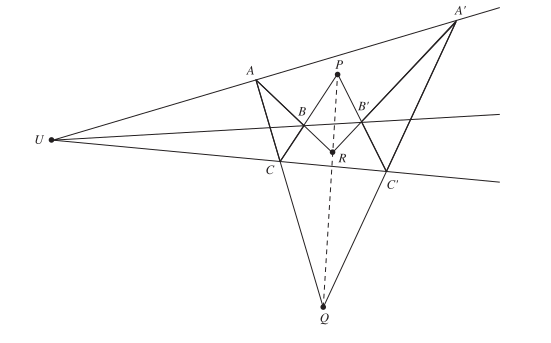
\includegraphics[width=0.75\linewidth]{pictures/desargues.png}
  \caption{Figure from \cite{brannan}.}
\end{figure}

\begin{proof}
  We will prove the theorem for the special case where $A=[1:0:0]$, $B=[0:1:0]$, $C=[0:0:1]$,
  and $U=[1:1:1]$. From the fundamental theorem of projective geometry, we know that it will be
  congruent to any other configuration. We can use the fact that projective congruence preserves
  projrctive properties, to deduce that the theorem holds in general.

  The line $AU$ has the equation $y=z$. Since $A'$ lies on $AU$, it must have coordinates
  $[a:b:b]$, where $b\ne 0$, since $A'\ne A$. We can also wirte $A'=[p:1:1]$, where $p=a/b$.
  Similary, $B'=[1:q:1]$, and $C'=[1:1:r]$.

  Now to find the point $P$, we find the equation of the line $BC$.
  \[
    \begin{vmatrix}
      x & y & z\\
      1 & q & 1\\
      1 & 1 & r
    \end{vmatrix}
    =0\Longrightarrow (qr-1)x-(r-1)y+(1-q)=0
  \]
  Substituting $x=0$ in the equation for the line $B'C'$, we get $(r-1)y=(1-q)z$, which immplies
  $P=[0:1-q:r-1]$. Similarly we find that $Q=[1-p:0:r-1]$, and $R=[1-p:q-1:0]$.

  To check the colinearity of $P$, $Q$, and $R$:
  \[
    \begin{vmatrix}
      0   & 1-q & r-1 \\
      1-p & 0   & r-1\\
      1-p & q-1 & 0
    \end{vmatrix}
  \]
  \begin{eqnarray*}
    &=& -(1-q)(1-p)(1-r)+(r-1)(1-p)(q-1)\\
    &=& 0
  \end{eqnarray*}

  i.e $P$, $Q$, and $R$ are colinear.
\end{proof}

Proof adapted from \cite{brannan}.

\begin{prop}
  There is a unique projective conic through any given set of five points.
\end{prop}

\begin{proof}
\end{proof}

Proof adapted from \cite{brannan}.

\begin{remark}
  \textbf{The Standard Projective Conic}\\
\end{remark}

\begin{prop}
  Let $E_1$ and $E_2$ be non-degenrate conics that pass through the points $P_1$, $Q_1$, $R_1$
  and $P_2$, $Q_2$, $R_2$ respectively. THen ther exists a projective transformation $t$ which
  maps $E_1$ to $E_2$ such that $t(P_1)=P_2$, $t(Q_1)=Q_2$, and $t(R_1)=R_2$.
\end{prop}

Proof adapted from \cite{brannan}.

\begin{theorem}[Pascal's Theorem]
\end{theorem}

\begin{figure}[H]
  \center
  
\includegraphics[width=\linewidth]{pictures/pascal.png}
  \caption{Figure from \cite{brannan}.}
  \label{fig:pascal}
\end{figure}

\begin{proof}
\end{proof}

Proof adapted from \cite{brannan}.

\section{The Cross-Ratio}

\begin{definition}
  Let $a$, $b$, $c$ and $d$ be four points on a projective line $D$. There exists a unique map
  from $D$ to $K\cup\{\infty\}$ that maps $a$ to $\infty$, $b$ to $0$, and $c$ to $1$. The
  image of $d$ under this projective mapping is called the \textit{cross-ratio} of the points
  $(a,b,c,d)$, and denoted $[a,b,c,d]$.
\end{definition}

\begin{prop}
  Let $a_1$, $a_2$, $a_3$, and $a_4$ be four points on the line $D$ (the first three being
  distinct) and $a'_1$, $a'_2$, $a'_3$, and $a'_4$ be four points on another line $D'$
  (satisfying the same assumption). There exists a projective transformation $f:D\rightarrow D'$
  such that $f(a_i)=a'_i$ iff $[a_1,a_2,a_3,a_4]=[a'_1,a'_2,a'_3,a'_4]$.
\end{prop}

\begin{proof}
  Assume $f$ is a projective mapping that sends $a_i$ to $a'_i$. Let 
\end{proof}

\section{Elliptic Curves}

\begin{definition}
  An elliptic curve is a non-empty, non-singular, degree 3 projective curve. \cite{spallone}
\end{definition}

\subsection{Group Laws on Conics}
